% 24th, Jan, 2001 Ver.1     Tatsuya Okabe
%                 Ver.2
%                 Ver.3
%                 Ver.4
%                 Ver.5
%
%---------------------------------------------------------------------------%
% Made by Tatsuya Okabe ( HONDA R&D Europe ( Deutschland ) GmbH )           %
% Checked by Bernhard Sendhoff ( HONDA R&D Europe ( Deutschland ) GmbH )    %
%---------------------------------------------------------------------------%
% Class DiffGeometric

\section{Abstract}

\noindent
With the class {\em DiffGeometric}, the ``Differentiative Geometiric
distribution'' can be simulated. To calculate this distribution, class
{\em Geometiric} is used twice. After getting two variables from {\em
Geometric}, the random number of {\em DiffGeometirc} is
calculated. This distribution is given by the following equation.

\vspace*{10mm}

\begin{equation}
f(x) = \frac{p \times (1-p)^x}{2-p}
\end{equation}

\vspace*{10mm}

\begin{center}
\begin{figure}[h]
\rotatebox{-90}{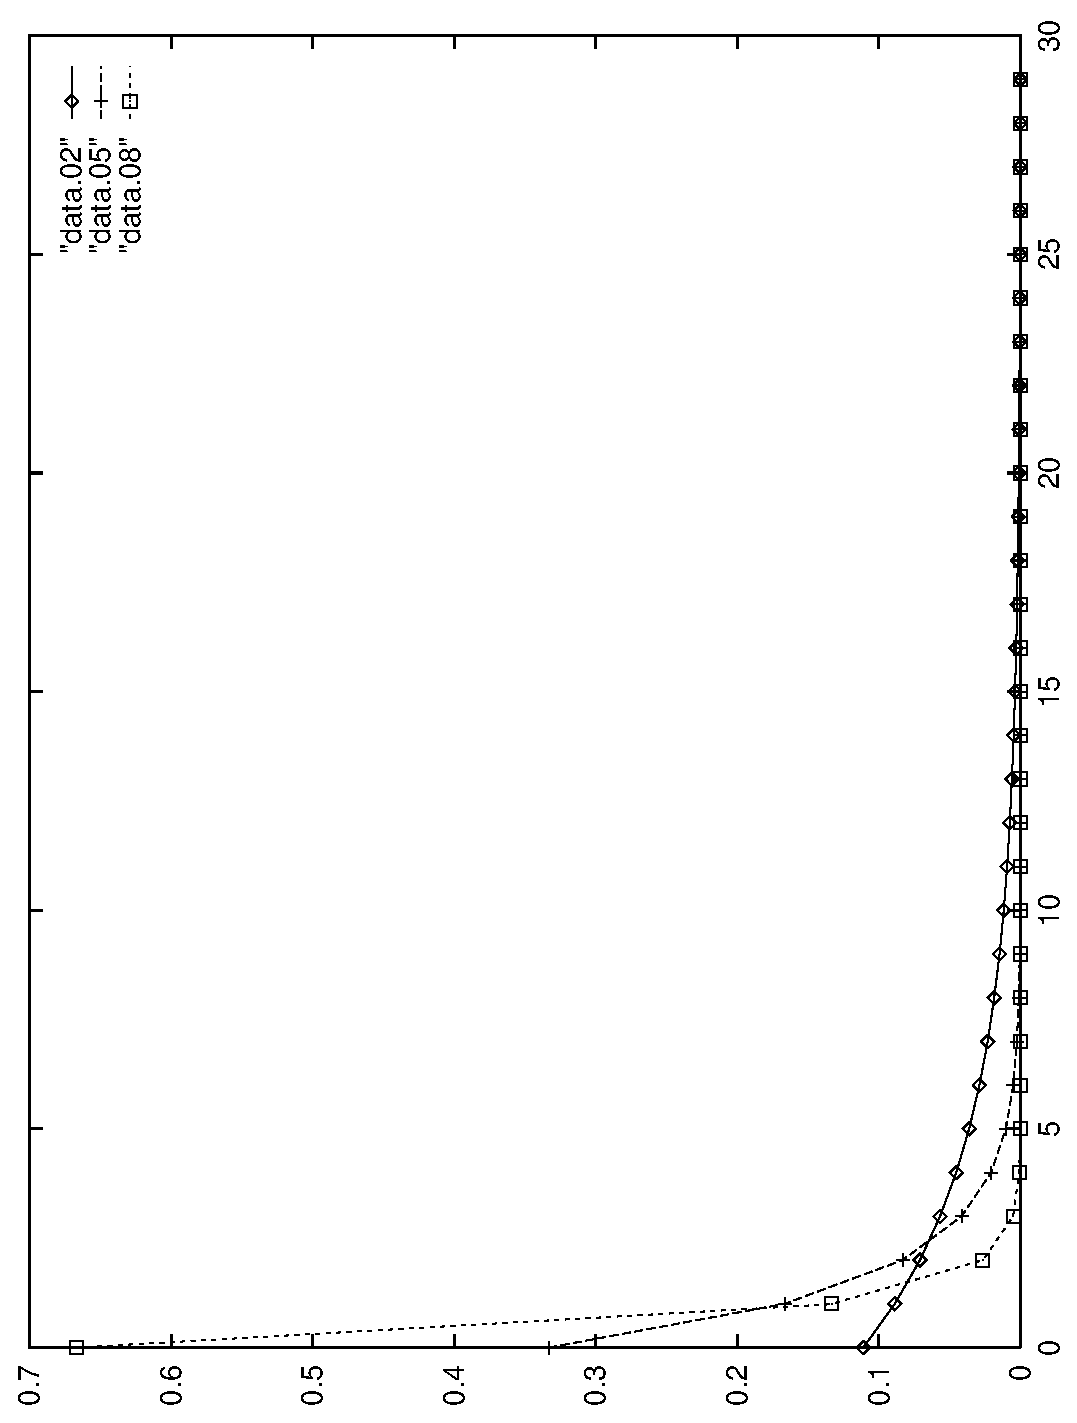
\includegraphics[height=12cm]{diffGeometric.eps}}\\
\caption{The DiffGeometiric distribution with $p = 0.8$ , $0.5$
and $0.2$.}
\end{figure}
\end{center}

\clearpage

\section{Public Methods}

\noindent
These methods can be used by all \cpp - programs, that have included the
header file DiffGeometric.h and the library EA.

\subsection{Constructors}

%---------------------------------------------------------------------------%
% 001
\index{DiffGeometric!( double mean )} 
\setNormalInstance
\printMethodWithOneParam
{}
{DiffGeometric}
{double}
{mean}
{The probability.}
{The default constructor. Generates the random generator of
Differential Geometric distribution.}
{None.}
{None.}
%---------------------------------------------------------------------------%

%---------------------------------------------------------------------------%
% 002
\index{DiffGeometric!( double mean, RNG\& r )}
\setNormalInstance
\setCorrectWidthThree{8pt}
\setParamOne{mean}{double}{The probability.} 
\setParamTwo{r}{RNG\&}{RNG class.}
\printMethodWithParamsSaved
{}
{None.}
{DiffGeometric}
{The constructor. Generates the random generator of Differential
Geometric distribution.}
{None.}
\setCorrectWidthThree{4pt}
%---------------------------------------------------------------------------%

\vspace*{10mm}

\subsection{Operators}

%---------------------------------------------------------------------------%
% 003
\index{operator( )!( double mean )} 
\setNormalInstance
\printMethodWithOneParam
{long}
{operator( )}
{double}
{mean}
{The probability.}
{Gets the result of Differential Geometric distribution.}
{The result of Differential Geometric distribution.}
{None.}
%---------------------------------------------------------------------------%

\clearpage

%---------------------------------------------------------------------------%
% 004
\index{operator( )!( )} 
\setNormalInstance
\printEmptyMethodReturnSpecial
{long}
{operator( )}
{Gets the result of Differential Geometric distribution.}
{The result of Differential Geometric distribution.}
{None.}
%---------------------------------------------------------------------------%

\vspace*{10mm}

\subsection{The probability}

%---------------------------------------------------------------------------%
% 007
\index{p!( const long\& x )} 
\setConstInstance
\printMethodWithOneParam
{double}
{p}
{const long\&}
{x}
{The factor which you want to calculate the probability.}
{Returns the probability of {\em x}.}
{The probability.}
{None.}
%---------------------------------------------------------------------------%


